\documentclass[12pt,a4paper,oneside]{book}
\usepackage[utf8]{inputenc}
\usepackage{amsmath}
\usepackage{amsfonts}
\usepackage{amssymb}
\usepackage{graphicx}
\usepackage[hidelinks]{hyperref}
\usepackage{minted}
\usepackage{tcolorbox}
\usepackage{geometry}
\usepackage{fancyhdr}
\usepackage{titlesec}
\usepackage{xcolor}
\usepackage{tikz}
\usetikzlibrary{shapes.geometric, arrows.meta, positioning}

% Setup page geometry
\geometry{
    a4paper,
    left=25mm,
    right=25mm,
    top=25mm,
    bottom=25mm
}

\setlength{\headheight}{14.5pt}

% Setup colors
\definecolor{primary}{RGB}{41, 128, 185}
\definecolor{secondary}{RGB}{142, 68, 173}
\definecolor{darkgray}{RGB}{50, 50, 50}

% Header and Footer
\pagestyle{fancy}
\fancyhf{}
\fancyhead[L]{\textcolor{primary}{\textbf{Generative AI Engineering Handbook}}}
\fancyhead[R]{\thepage}
\renewcommand{\headrulewidth}{0.4pt}
\renewcommand{\footrulewidth}{0.4pt}

% Title formats
\titleformat{\chapter}[display]
  {\normalfont\huge\bfseries\color{primary}}{\chaptertitlename\ \thechapter}{20pt}{\Huge}
\titleformat{\section}
  {\normalfont\Large\bfseries\color{secondary}}{\thesection}{1em}{}

% Custom boxes
\tcbuselibrary{minted,skins,breakable}
\newtcolorbox{infobox}[1][]{breakable,colback=blue!5!white,colframe=blue!75!black,fonttitle=\bfseries,title=#1}
\newtcolorbox{warningbox}[1][]{breakable,colback=red!5!white,colframe=red!75!black,fonttitle=\bfseries,title=#1}
\newtcolorbox{bestpractice}[1][]{breakable,colback=green!5!white,colframe=green!75!black,fonttitle=\bfseries,title=#1}
\newtcolorbox{concept}[1][]{breakable,colback=purple!5!white,colframe=purple!75!black,fonttitle=\bfseries,title=#1}
\newtcolorbox{tipbox}[1][]{breakable,colback=orange!5!white,colframe=orange!75!black,fonttitle=\bfseries,title=Tip: #1}

\newtcblisting{codeblock}[2]{
    breakable,
    colback=black!80!white,
    colframe=black!80!white,
    coltitle=white,
    fonttitle=\bfseries,
    title=#1,
    listing only,
    minted language=#2,
    minted style=monokai,
    minted options={linenos,breaklines,fontsize=\small}
}

\title{\Huge \textbf{Generative AI Engineering Handbook} \\ \vspace{0.5cm} \Large The Definitive Guide for Production Systems}
\author{Synthesized from Scaler Academy}
\date{\today}

\begin{document}

\maketitle
\tableofcontents
\newpage

\chapter{Introduction to GenAI}
\section{The GPT Paradigm}
The term \textbf{GPT} stands for \textbf{Generative Pre-trained Transformer}.

Think of traditional programming like a calculator: you input $2+2$, and it always gives exactly $4$. It is $100\%$ predictable.

Generative AI works very differently. It acts like the world's most advanced "autocomplete" feature on your phone keyboard. It has read millions of books and articles (its "pre-training"). So, its only job is to look at the words you just typed and \textit{predict} what the next logical word should be. It does this over and over again to write full sentences!

This text-generation magic was made possible by the \textbf{"Attention Is All You Need"} research paper by Google.

\section{Deep Dive: Tokenization}
Computers only understand numbers (0s and 1s); they don't understand English words like "Hello." So, how does an AI read our text? Through \textbf{Tokenization}.

\begin{figure}[h!]
\centering
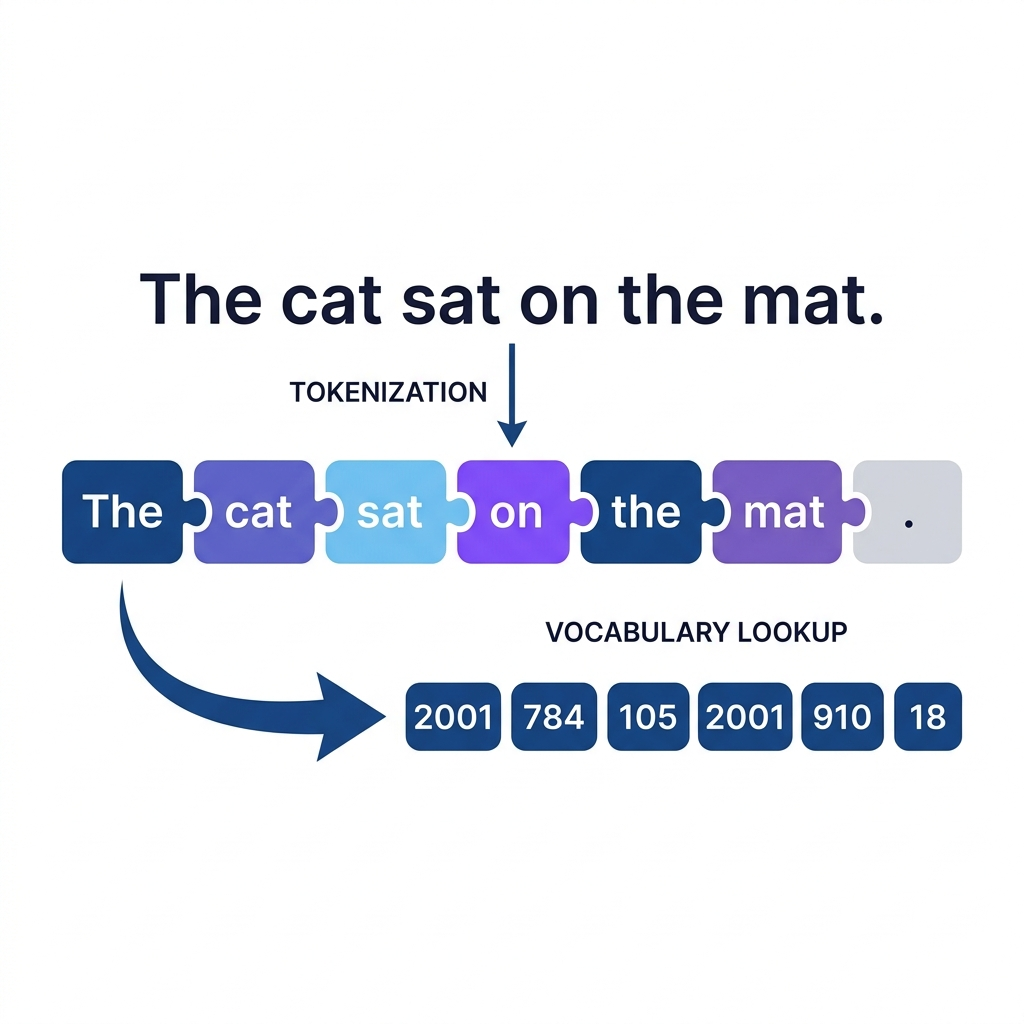
\includegraphics[width=0.8\textwidth]{../images/tokenization.png}
\caption{Visualizing the Tokenization Process}
\end{figure}

Instead of reading letter-by-letter, the AI groups text into small chunks called \textbf{tokens}. You can think of a token like a single puzzle piece. Sometimes a token is a whole word (like "apple"), and sometimes it's just a syllable. The AI converts these puzzle pieces into numbers so the computer can process them.

\begin{codeblock}{Tokenization in Node.js}{javascript}
	// Importing a common tokenizer library
	import { get_encoding } from "tiktoken";

	// Convert input string into semantic tokens
	const encoder = get_encoding("cl100k_base");
	const tokens = encoder.encode("Hello, how are you?");
	console.log(tokens); // Output: [9906, 11, 4919, 527, 499, 30]
\end{codeblock}

\section{Input Embeddings \& Dimensionality}
Now that the computer has numbers (tokens), it needs to understand what those numbers actually \textit{mean}. This is done using \textbf{Input Embeddings}.

\begin{figure}[h!]
\centering
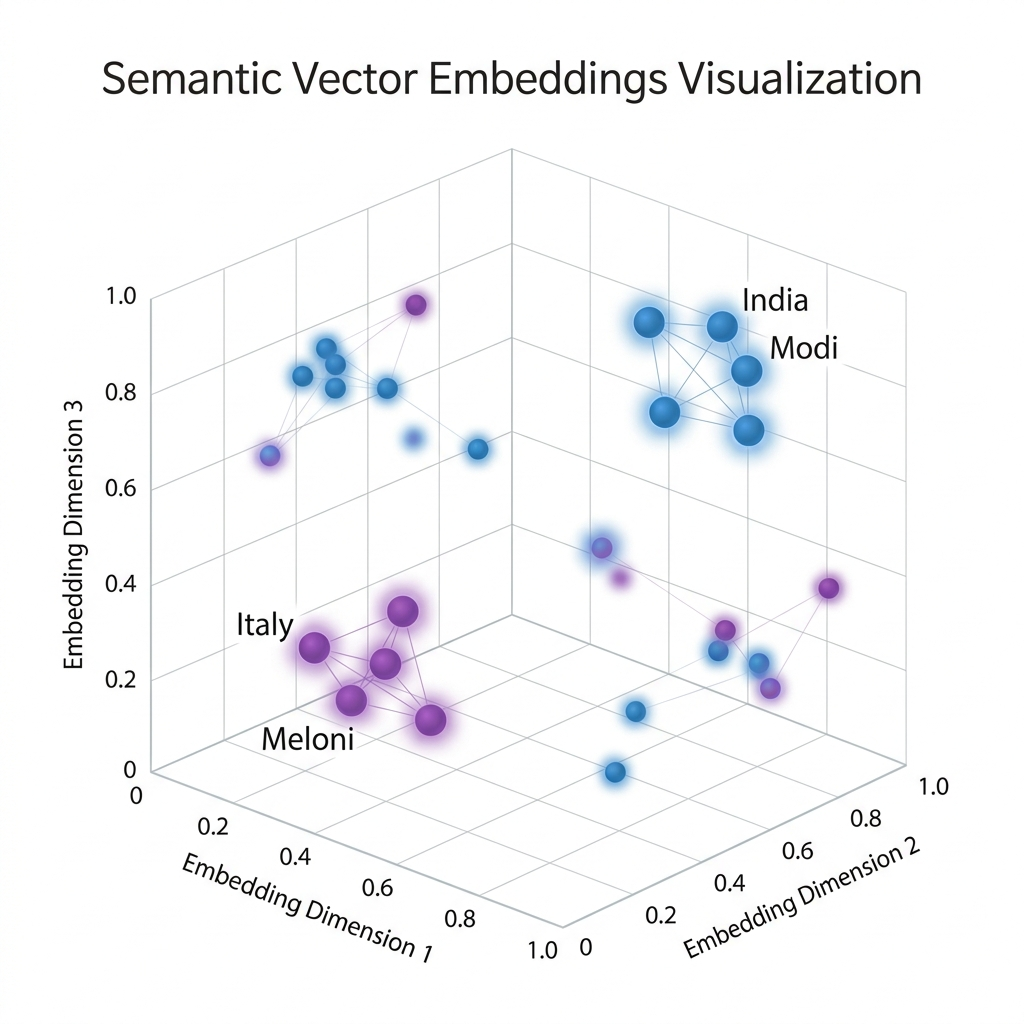
\includegraphics[width=0.8\textwidth]{../images/vector_embeddings.png}
\caption{Words mapped in a 3D Semantic Vector Space}
\end{figure}

Imagine a massive 3D map of concepts in the AI's brain. On this map, the word "Modi" is placed very close to "India". The word "Meloni" is placed close to "Italy". By turning words into coordinates on this map (called vectors), the AI mathematically understands that certain words are deeply related to each other!

\begin{concept}{Vector Dimensions}
	A normal map is 2D (Latitude and Longitude). But AI maps are incredibly complex. A standard model (like OpenAI's) plots words on a map with \textbf{1,536 dimensions}! This massive size allows the AI to capture very subtle differences in meaning, like the difference between a "bank" (for money) and a river "bank".
\end{concept}

\begin{codeblock}{Generating Embeddings (OpenAI SDK)}{javascript}
	import OpenAI from "openai";
	const openai = new OpenAI({ apiKey: process.env.OPENAI_API_KEY });

	const response = await openai.embeddings.create({
			model: "text-embedding-3-small",
			input: "Generative AI is revolutionary.",
		});
	console.log(response.data[0].embedding); // Array of 1536 floats
\end{codeblock}

\section{Positional Encoding}
If you give the AI the words "dog", "bit", and "man", it needs to know the exact order. "The dog bit the man" is very different from "The man bit the dog"!

\textbf{Positional Encoding} is a technique that attaches a hidden "timestamp" or "tag" to each word, so the AI knows exactly what order the words appeared in.

\begin{tipbox}[Open-Source Alternatives: Ollama]
	While OpenAI and Anthropic are industry standards, API costs accumulate rapidly. For local, zero-cost development, you can host open-source LLMs natively on your machine using \textbf{Ollama}.
\end{tipbox}

\chapter{Prompt Engineering}

\section{The GIGO Principle}
In computer science, there is a famous rule: \textbf{Garbage In, Garbage Out (GIGO)}.

Think of it like a recipe app. If you input terrible ingredients, the app will give you a terrible recipe. The exact same rule applies to LLMs. If your prompt is vague or missing context, the AI will give you a bad answer. Good output tokens require good input tokens.

\section{The Goldfish Memory (Statelessness)}
When you use an LLM, you might feel like you are having a continuous conversation. You are not.

LLMs have the memory of a goldfish. They are entirely \textbf{stateless}. Every single time you press "Send", the AI forgets everything you previously talked about. To fix this, developers must package your \textit{entire} chat history and send it back to the AI with every single new message.

\begin{infobox}[Cost Efficiency: Cached Tokens]
	Sending massive chat histories repeatedly sounds incredibly expensive. However, providers like OpenAI aggregate these historical messages and bill them at a massive discount as \textbf{Cached Tokens}, making long conversations financially viable.
\end{infobox}

\section{The Universal Adapter: ChatML Format}
Historically, every AI company had a completely different way of accepting prompts. Some used \texttt{<instructions>} tags, others used \texttt{Question/Answer} formats.

Then, OpenAI introduced the \textbf{ChatML format}. It organizes conversations into an array of objects, where each object has a \texttt{role} and \texttt{content}.

\begin{concept}{The "USB-C" of the AI World}
	ChatML became so popular that it essentially became the "USB-C" port of the AI industry. Today, competitors like DeepSeek, Claude, and Gemini have built their APIs to accept OpenAI's exact ChatML format. This means developers can switch AI providers without rewriting any code!
\end{concept}

\section{The AI's Boss: System Prompts}
Within the ChatML format, there are different roles (User, Assistant, System). The most important is the \textbf{System Prompt}.

Think of the System Prompt as the AI's strict "Project Manager" or "Boss." It gives the AI a persona and strict operational boundaries.

\begin{codeblock}{Restricting AI Behavior (System Prompt)}{javascript}
	const messages = [
	{
			role: "system",
			content: "You are an expert in JavaScript. You only know JavaScript. If the user asks about Python, refuse to answer."
		},
	{
			role: "user",
			content: "Can you write a poem about a dog in Python?"
		}
	];
	// The AI will refuse, because its "Boss" told it not to!
\end{codeblock}

\section{Prompting Styles}
Depending on the complexity of your task, there are several standard "styles" or techniques for prompting an LLM:

\begin{itemize}
	\item \textbf{Zero-Shot Prompting:} Asking the model to perform a task without providing any examples. The model relies entirely on its pre-trained knowledge.
	\item \textbf{Few-Shot Prompting:} Providing the model with a few examples (e.g., Question and Answer pairs) within the prompt to teach it the desired output format or pattern before asking the final question.
	\item \textbf{Chain of Thought (CoT) Prompting:} Instructing the model to break down complex reasoning tasks into intermediate steps (e.g., adding "Think step-by-step" to the prompt). This drastically improves performance on logic and math problems.
\end{itemize}

\begin{tipbox}[Further Reading]
	For an exhaustive, definitive guide on advanced prompt engineering techniques, I highly recommend exploring the \href{https://www.promptingguide.ai/}{Prompt Engineering Guide (promptingguide.ai)}.
\end{tipbox}

\chapter{Introduction to AI Agents}

\section{The "Frozen in Time" Problem}
LLMs are brilliant, but they have a massive flaw: they are frozen in time. If you ask an LLM, "What is the weather in Delhi right now?", it will fail because its knowledge is limited to its pre-training data.

To solve this, we cannot just retrain the LLM daily (that costs millions of dollars). We also cannot fetch the weather of \textit{every} city on Earth and shove it into the prompt (that wastes thousands of tokens).

The solution? \textbf{Agentic AI}.

\section{The Brain and Body Analogy}
To understand Agentic AI, think of the human body:
\begin{itemize}
	\item \textbf{The Body (APIs \& Functions):} Traditional microservices are like hands and legs. They can perform actions (like fetching live weather or booking a flight ticket), but they \textit{cannot think}.
	\item \textbf{The Brain (LLMs):} Large Language Models are like a brain. They can think, reason, and write poetry, but they have no hands to \textit{perform actions}.
\end{itemize}

An \textbf{AI Agent} connects the brain to the body. It gives the LLM "hands and legs" to interact with the real world!

\section{Tool Calling \& Chain of Thought}
How do we connect the brain to the hands? Through \textbf{Tool Calling}.

\begin{figure}[h!]
\centering
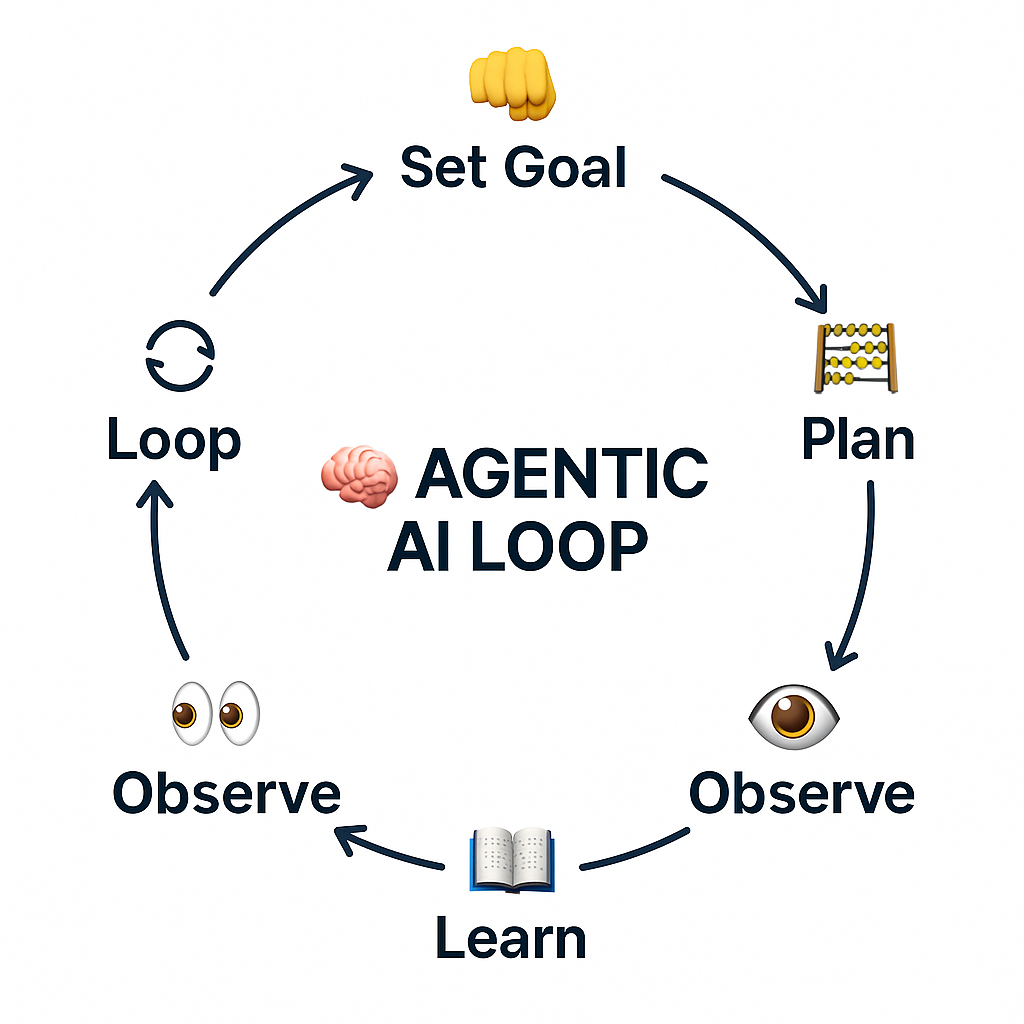
\includegraphics[width=0.8\textwidth]{../images/agentic_loop.png}
\caption{The Agentic Action Loop (Think $\rightarrow$ Act $\rightarrow$ Observe)}
\end{figure}

Developers write simple local functions (like \texttt{getWeather(city)}). They pass a description of this function to the LLM. The LLM cannot magically run the code itself. Instead, it enters a \textbf{Chain of Thought} thinking loop:

\begin{concept}{The Agentic Loop}
	\texttt{Start} $\rightarrow$ \texttt{Think} ("I need the weather") $\rightarrow$ \texttt{Tool Call} ("Developer, please run the getWeather tool for Delhi") $\rightarrow$ \texttt{Observe} ("The developer gave me the result: 33°C") $\rightarrow$ \texttt{Output} ("The weather is 33°C!").
\end{concept}

\section{The Danger Zone: Guardrails}
Because an agent can execute code, it is incredibly powerful. For example, AI tools like Cursor give the LLM access to your terminal to create files and folders.

But this is dangerous! What if the LLM hallucinates and calls a tool to delete your entire hard drive?

\begin{warningbox}[LLM-as-a-Judge]
	Never let an LLM execute destructive commands blindly. Production systems implement \textbf{Guardrails}. Before executing a dangerous tool call, pass the LLM's "thought" to a secondary, smaller LLM that acts as a security guard to evaluate if the action is safe.
\end{warningbox}

\chapter[RAG 1 – Intro to RAG]{RAG 1 – Introduction To\\Retrieval-Augmented Generation}

\section{The Lawyer's Problem}
Imagine a lawyer with 3,000 private case files. An LLM has never seen these files because they aren't on the public internet. If the lawyer asks the LLM a question about "Case 420," it will hallucinate.

How do we fix this?
\begin{itemize}
	\item \textbf{Brute Force 1:} Stuff all 3,000 files into the system prompt. (Fails due to Context Window limits and massive token costs).
	\item \textbf{Brute Force 2:} Pass the files one-by-one to a Small Language Model and ask "Is this relevant?" (Fails because iterating through 3,000 files via an API takes hours).
\end{itemize}
The elegant solution is \textbf{Retrieval-Augmented Generation (RAG)}.

\section{Semantic Meaning \& Vector Embeddings}
When you hear the word "Modiji," you instantly think of "Prime Minister" or "India." Words have deep, hidden connections called semantic meaning.

LLMs encode these semantic meanings into mathematical coordinates called \textbf{Vector Embeddings}. If two sentences have similar meanings, their coordinates will be placed very close together in a mathematical graph.

\section{Step 1: The Indexing Pipeline}
Before the user can even ask a question, we must prepare the lawyer's files.
\begin{enumerate}
	\item \textbf{Loading:} We read the 3,000 PDF files (using tools like Langchain's \texttt{PDFLoader}).
	\item \textbf{Chunking:} A full book is too much to process at once, so we tear it into individual pages (chunks).
	\item \textbf{Embedding:} We use an embedding model (like \texttt{text-embedding-3}) to convert each text chunk into a mathematical vector.
	\item \textbf{Storing:} We place the Vector and the Text Chunk into a special filing cabinet known as a \textbf{Vector Database} (e.g., Qdrant, Pinecone, ChromaDB).
\end{enumerate}

\begin{tipbox}[Chunking Strategies]
	Chunking is a complex engineering problem. For a deep dive into fixed-size, sentence-based, and semantic chunking methods, read Pinecone's \href{https://www.pinecone.io/learn/chunking-strategies/}{Chunking Strategies Guide}.
\end{tipbox}

\begin{figure}[!ht]
    \centering
    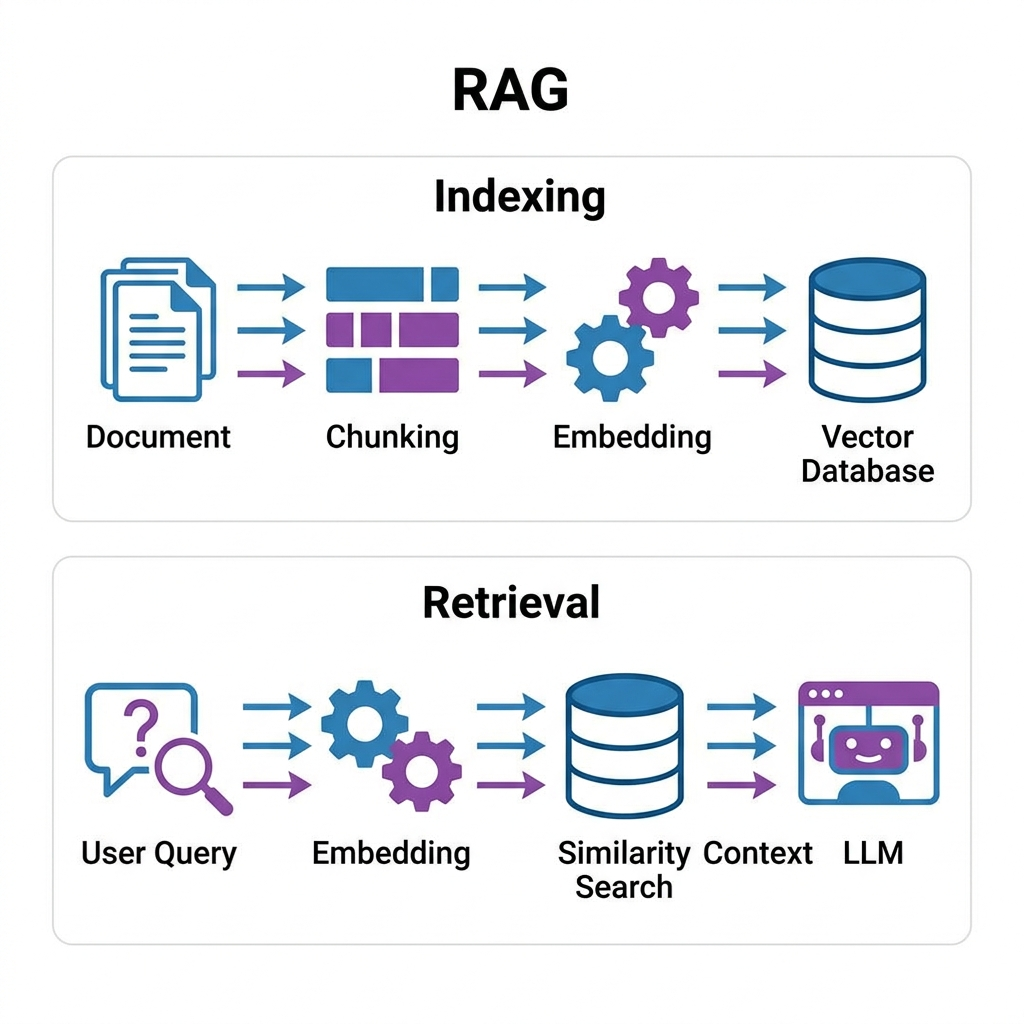
\includegraphics[width=\textwidth]{../images/rag_pipeline.png}
    \caption{The Indexing and Retrieval Pipelines in a RAG Architecture.}
    \label{fig:rag_pipeline}
\end{figure}

\section{Step 2: The Retrieval Pipeline}
Now, the lawyer asks a question!
\begin{enumerate}
	\item We convert the lawyer's question into a Vector using the \textit{exact same} embedding model.
	\item We do a \textbf{Similarity Search} in our Vector Database: "Find the top 3 chunks closest to this question's coordinates."
	\item The database returns those 3 specific chunks.
	\item We pass \textit{only} those 3 chunks to the main LLM to generate the final answer. Fast, cheap, and accurate!
\end{enumerate}

\chapter{RAG 2 – Advanced Retrieval Strategies}

\section{The Production Problem: GIGO}
Basic RAG looks great in a tutorial, but it fails in production. Why? \textbf{Garbage In, Garbage Out (GIGO)}.
\begin{itemize}
	\item \textbf{Garbage Indexing:} If a user uploads a terrible, messy PDF, the chunks will be terrible. We can't control this.
	\item \textbf{Garbage Retrieval:} Users rarely know what to search for. They make typos (e.g., "how to dubug nod sj"). It's like humming a tune on YouTube because you forgot the song's name. If the query is bad, the Vector Database returns bad chunks. We \textit{can} control this!
\end{itemize}

\begin{tipbox}[Accuracy is King]
	In RAG systems, \textbf{Accuracy} is the most important metric. We gladly trade a little bit of Speed and Cost (by adding extra processing steps) to ensure the user gets a highly accurate answer.
\end{tipbox}

\section{Pre-Retrieval: Query Translation}
Instead of taking the user's messy query directly to the Vector Database, we add a step \textit{before} the search.

We pass the raw query to a Small Language Model (SLM) that acts like a smart librarian. Its job is to fix typos and add technical context.
\begin{itemize}
	\item \textbf{User Types:} "dubug nod sj"
	\item \textbf{SLM Translates To:} "How to perform debugging in Node.js"
\end{itemize}
Now, when we search the Vector Database using the \textit{translated} query, the chunks we get back are incredibly accurate!

\section[Corrective RAG]{Post-Retrieval: Corrective RAG (CRAG)}
In the CRAG workflow, immediately after receiving the user query, we often perform \textbf{query translation using a Small Language Model (SLM)} to normalize the request before retrieval. What if the Vector Database still gives us a bad chunk? We use a self-correcting loop known as \textbf{Corrective RAG}.

\begin{concept}{LLM-as-a-Judge}
	After the Vector Database returns chunks, we don't blindly trust them. We ask an LLM: \textit{"Are these chunks actually relevant to the user's question?"}
	\begin{itemize}
		\item If \textbf{Yes}: We proceed to generate the final answer.
		\item If \textbf{No}: We throw the chunks in the trash, go back to the Query Translator, and tell it to rewrite the query again!
	\end{itemize}
\end{concept}

\begin{figure}[h!]
	\centering
	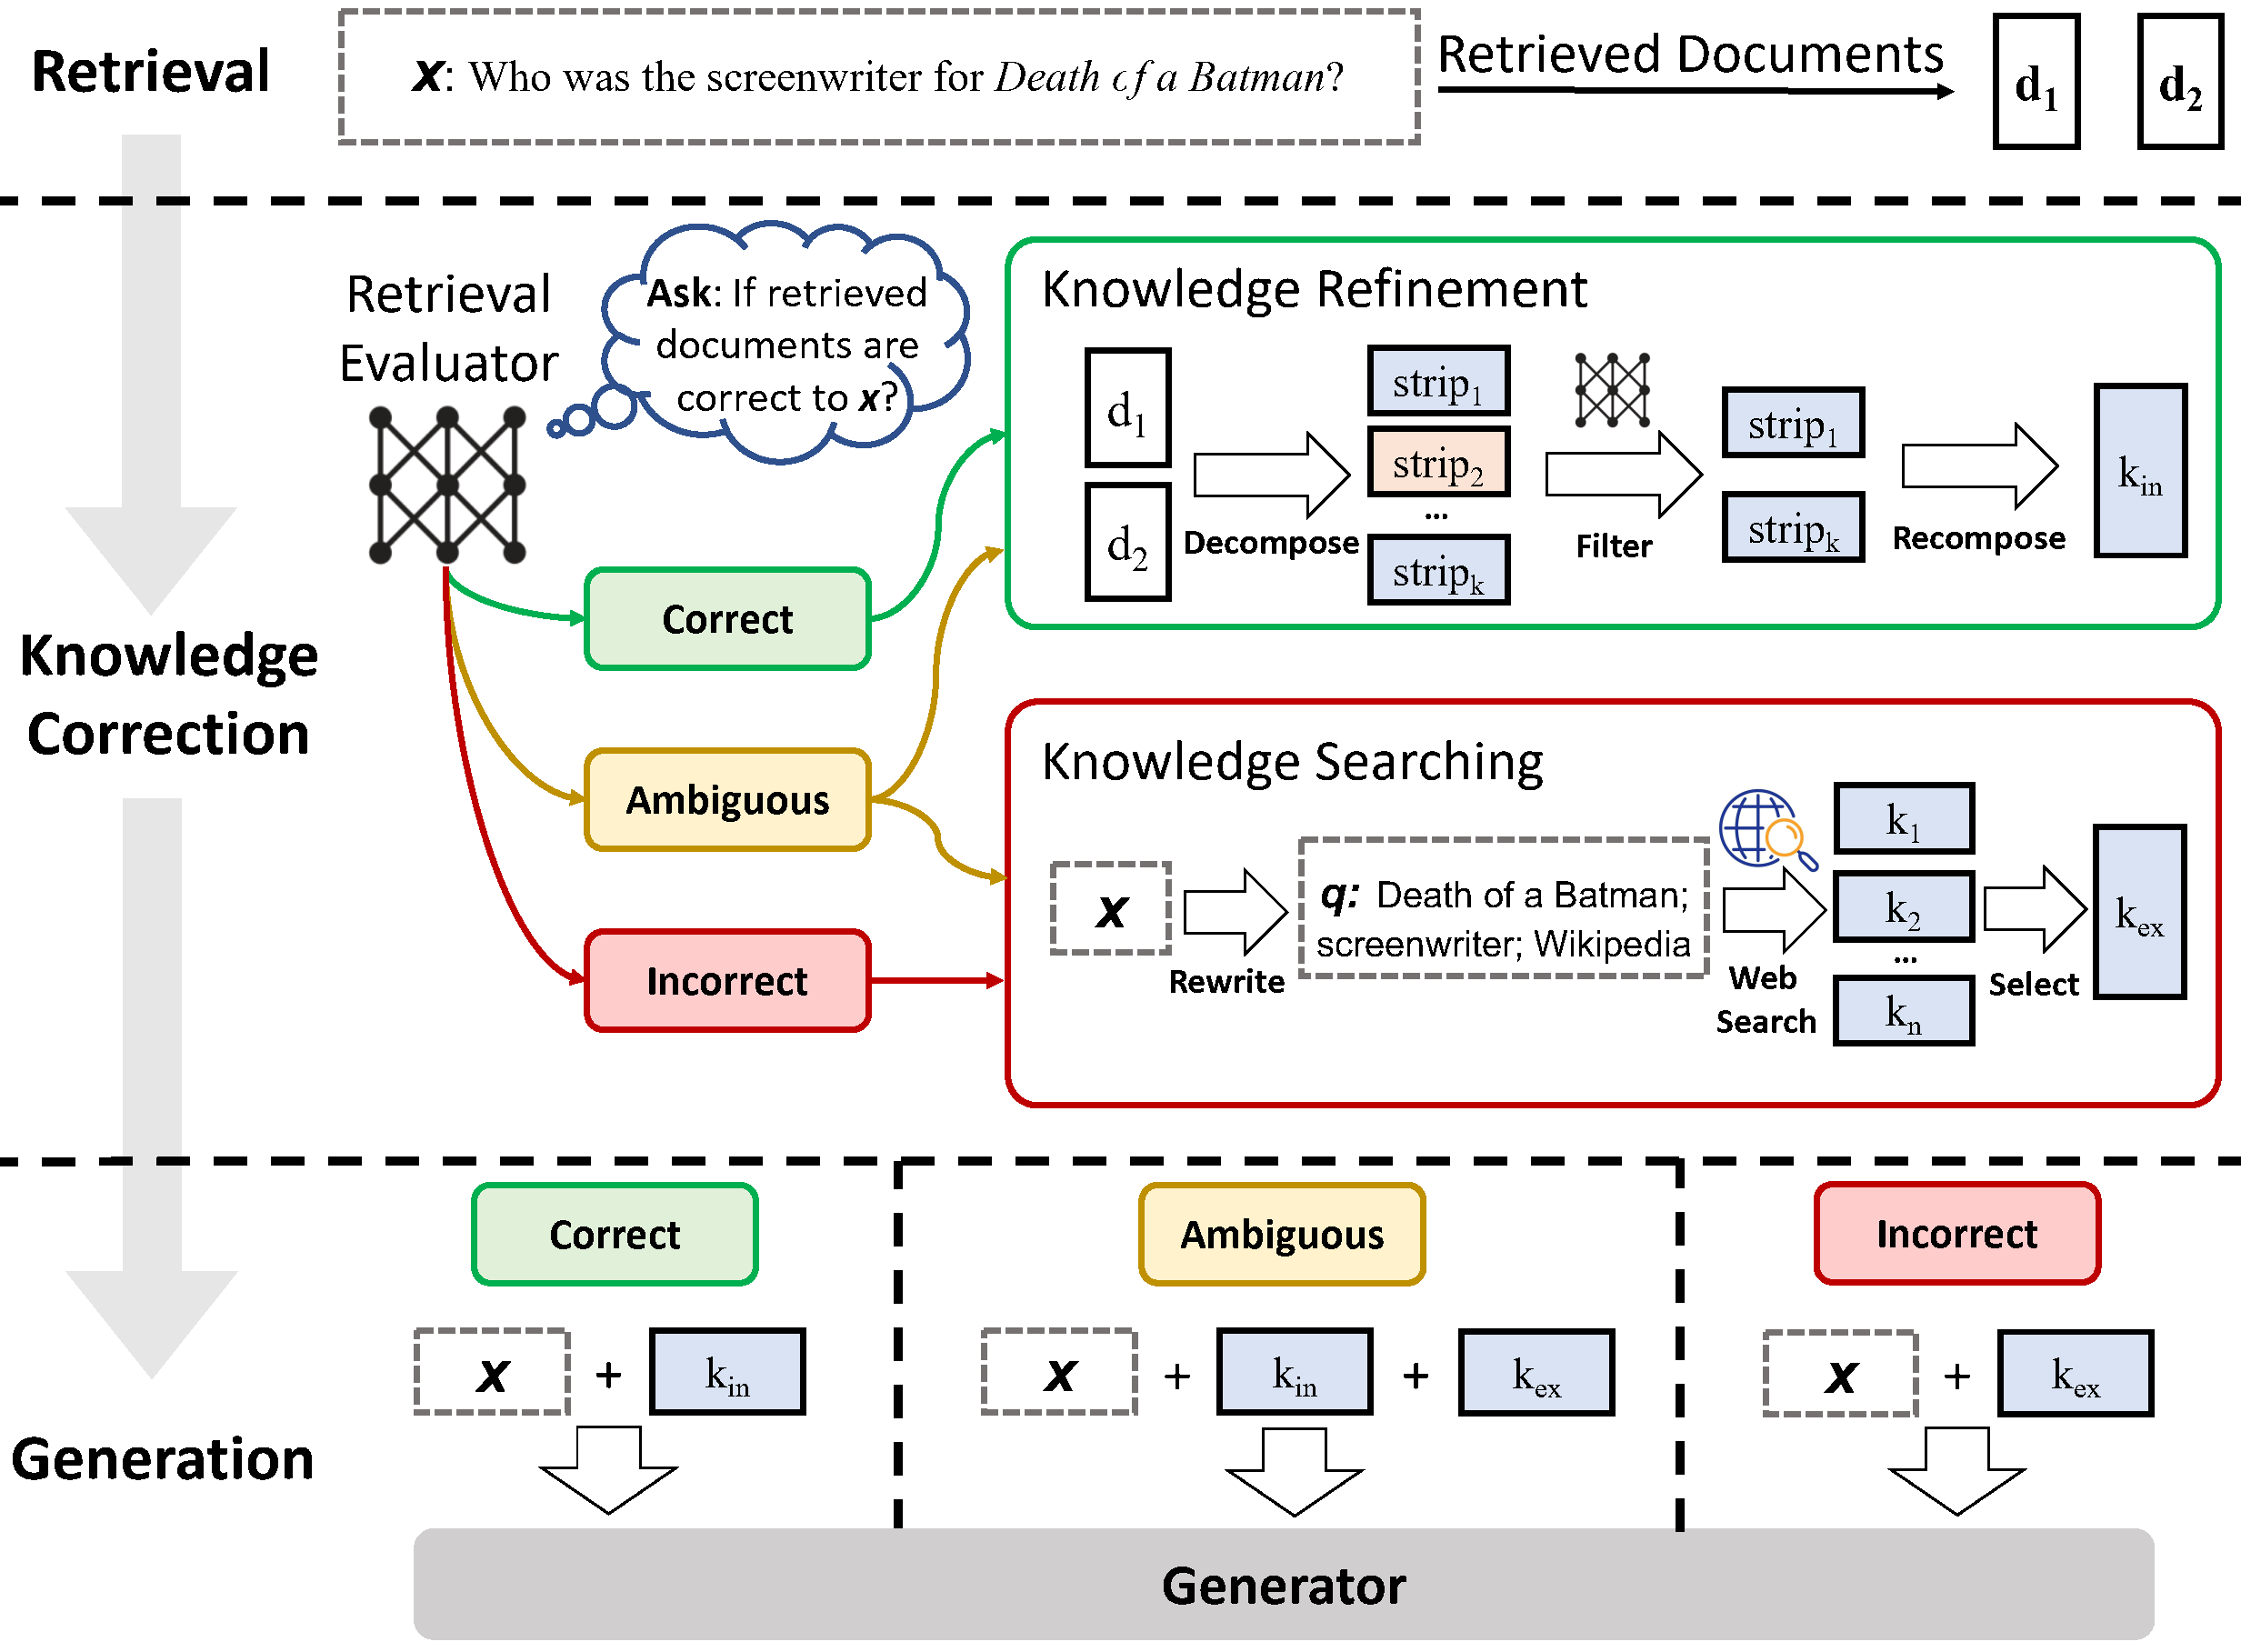
\includegraphics[width=\textwidth]{../images/crag_architecture.png}
	\caption{Corrective RAG (CRAG) Workflow Diagram}
\end{figure}

\section{Hypothetical Document Embeddings (HyDE)}

\begin{figure}[h!]
	\centering
	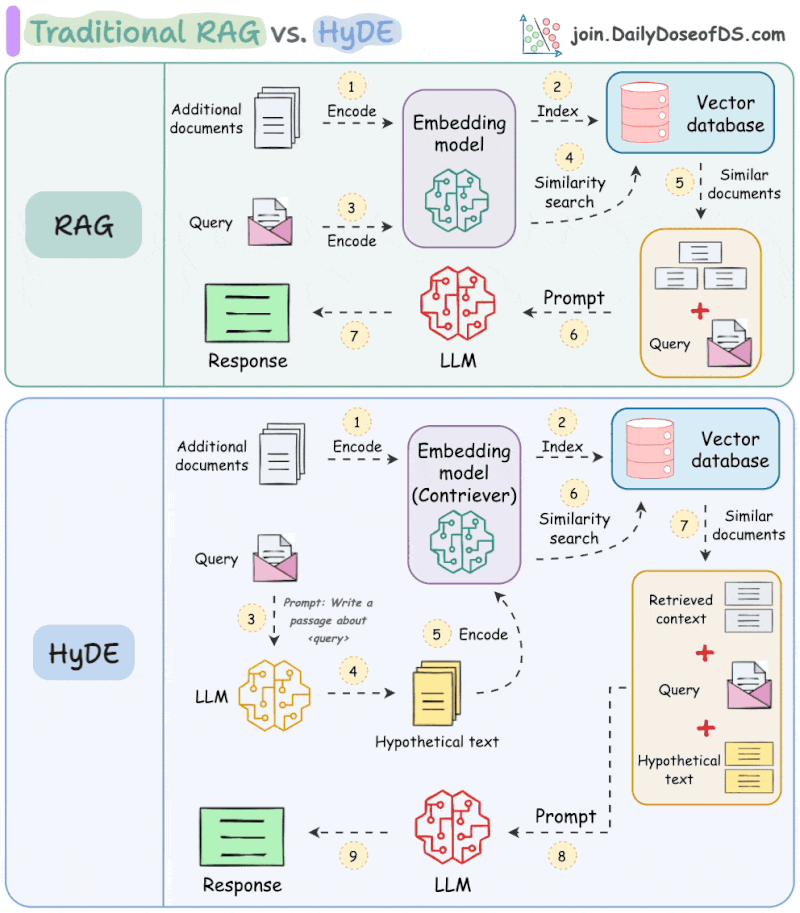
\includegraphics[width=\textwidth]{../images/rag_vs_hyde.png}
	\caption{Traditional RAG vs. HyDE Workflow Comparison}
\end{figure}

\begin{concept}{Document-to-Document Search}
	When a user asks a short question (e.g., "How long to remove a wisdom tooth?"), semantic search often fails. A short question structurally looks nothing like a long, detailed medical document. \textbf{HyDE} solves this by forcing a \textit{document-to-document} comparison.
	\begin{enumerate}
		\item \textbf{Generation:} The query is passed to an LLM to write a hypothetical answer passage.
		\item \textbf{Embedding:} Even if this fake document hallucinates facts, it captures the perfect vocabulary and structure. We embed this fake document instead of the query.
		\item \textbf{Retrieval:} The Vector DB easily finds real documents that look structurally identical to the fake document.
	\end{enumerate}
\end{concept}

\begin{figure}[h!]
	\centering
	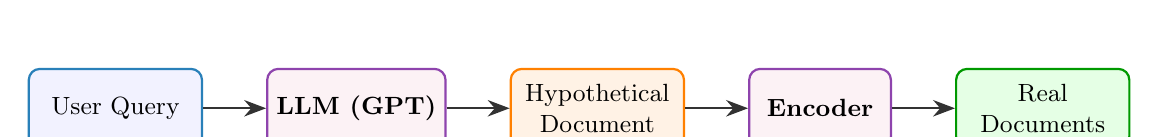
\begin{tikzpicture}[
		node distance=1cm and 0.8cm,
		box/.style={rectangle, draw=primary, fill=blue!5, thick, minimum width=2.2cm, minimum height=1cm, align=center, rounded corners, font=\small},
		model/.style={rectangle, draw=secondary, fill=purple!5, thick, minimum width=1.8cm, minimum height=1cm, align=center, rounded corners, font=\small\bfseries},
		arrow/.style={-{Stealth[scale=1.2]}, thick, draw=darkgray}
		]

		% Nodes
		\node[box] (query) {User Query};
		\node[model, right=of query] (gpt) {LLM (GPT)};
		\node[box, right=of gpt, fill=orange!10, draw=orange] (hypo) {Hypothetical\\Document};
		\node[model, right=of hypo] (encoder) {Encoder};
		\node[box, right=of encoder, fill=green!10, draw=green!60!black] (results) {Real\\Documents};

		% Arrows
		\draw[arrow] (query) -- (gpt);
		\draw[arrow] (gpt) -- (hypo);
		\draw[arrow] (hypo) -- (encoder);
		\draw[arrow] (encoder) -- (results);

	\end{tikzpicture}
	\caption{HyDE: Using fake documents to retrieve real documents}
\end{figure}

\chapter[LangChain \& LangGraph]{LangChain Fundamentals \\ \& LangGraph}

\section{The Problem: Losing Control}
Before AI, we wrote \textbf{Procedural Code}. We wrote Step 1, Step 2, and Step 3. As developers, we had 100\% control over exactly what our code would do.

When \textbf{Agentic AI} arrived, we gave our LLMs access to Tools. The LLM gained 100\% autonomy to decide \textit{which} tool to call and \textit{when} to call it. Developers suddenly lost control over their own applications!

\section{The Airplane vs. Train Analogy}
To understand LangGraph, think about travel:
\begin{itemize}
	\item \textbf{A Pure Agent is like an Airplane:} It can fly anywhere, in any direction, at any altitude. It is completely autonomous but highly unpredictable.
	\item \textbf{LangGraph is like a Train on Tracks:} It still drives itself, but it is strictly confined to the tracks (the graph) you built. It cannot go rogue. It must visit State A before State B.
\end{itemize}

\begin{figure}[!ht]
    \centering
    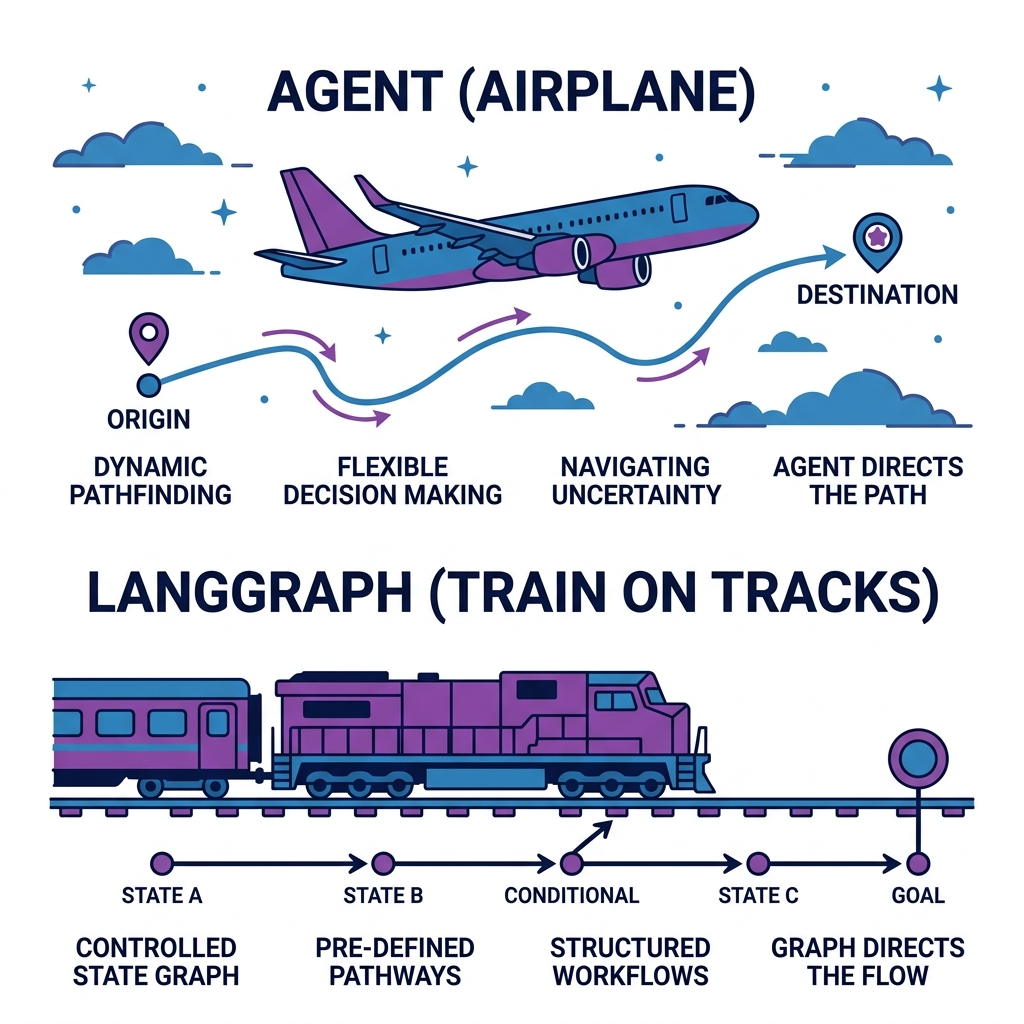
\includegraphics[width=\textwidth]{../images/langgraph_train.png}
    \caption{The autonomy of Pure Agents (Airplane) versus the predictability of LangGraph (Train).}
    \label{fig:langgraph_train}
\end{figure}

\section{Core LangGraph Components}
LangGraph uses scary academic terms, but they are actually very simple concepts:

\begin{itemize}
	\item \textbf{State (The Backpack):} A global memory object that gets passed around. As the agent completes tasks, it throws information into the backpack so it doesn't forget anything. (Similar to React's Context API or Redux).
	\item \textbf{Node (The Train Station):} A specific stop where work gets done (e.g., Calling an LLM, searching a Vector Database).
	\item \textbf{Edge (The Tracks):} The physical tracks connecting the train stations.
	\item \textbf{Conditional Edge (The Switch Track):} A junction where the LLM gets to decide which path to take. (\textit{e.g., "Is the database chunk good? If yes, travel to the Generate Answer station. If no, travel to the Rewrite Query station."})
\end{itemize}

\begin{codeblock}{LangGraph Workflow Concept}{python}
	from langgraph.graph import StateGraph, END

	# Create the Backpack (State)
	workflow = StateGraph(AgentState)

	# Build the Train Stations (Nodes)
	workflow.add_node("agent", call_agent)
	workflow.add_node("action", execute_tool)

	# Build the Switch Track (Conditional Edge)
	workflow.add_conditional_edges(
	"agent",
	should_continue,
	{
			"continue": "action",
			"end": END
		}
	)
\end{codeblock}

\section{LangSmith: Observability}
When you have a train running automatically, you need to monitor it. \textbf{LangSmith} is like Grafana for AI. It acts as a dashboard that tracks exactly which tools your agent is calling, how long it takes, and how much money (tokens) it is spending behind the scenes.

\begin{tipbox}[The Industry Shift]
	While LangGraph popularized this workflow, the AI industry is actively shifting \textit{away} from it. Major providers (like OpenAI and Google) have copied these orchestration features directly into their native \textbf{Agent SDKs}. We will focus on these modern SDKs in future chapters!
\end{tipbox}

\chapter{Agent SDK --- Fundamentals}

The industry is rapidly shifting away from complex orchestration graphs and toward native \textbf{Agent SDKs}. These SDKs abstract away the heavy "while-loop" boilerplate, allowing developers to build multi-agent systems using standard TypeScript or Python.

\section{The Microservices Analogy}
In modern backend development, you don't build one monolithic server. Instead, you build \textbf{Microservices} (e.g., an Authentication server, a Payments server). A user's request hits a \textbf{Gateway / Load Balancer}, which then routes the traffic to the correct server.

We apply this exact same logic to Agentic AI!
\begin{itemize}
	\item \textbf{Isolated Agents:} Instead of building one "God Agent" that tries to do everything, we build highly specialized agents (e.g., a Database Agent, a Coding Agent, a Cooking Agent).
	\item \textbf{The Gateway Agent:} The user's prompt is sent to a \textbf{Gateway Agent}. Its \textit{only} job is to read the prompt and route it to the correct specialized agent.
\end{itemize}

\begin{codeblock}{Creating a Specialized Agent}{typescript}
import { Agent } from "@openai/agents"; // Example SDK

const cookingAgent = new Agent({
    name: "Cooking Agent",
    instructions: "You are a master chef. Only answer questions about food.",
    model: "gpt-4o"
});
\end{codeblock}

\begin{tipbox}[Further Reading]
	For the official documentation on building with the OpenAI Agents framework, refer to their \href{https://github.com/openai/openai-agents-python}{GitHub Repository}.
\end{tipbox}

\begin{figure}[!ht]
    \centering
    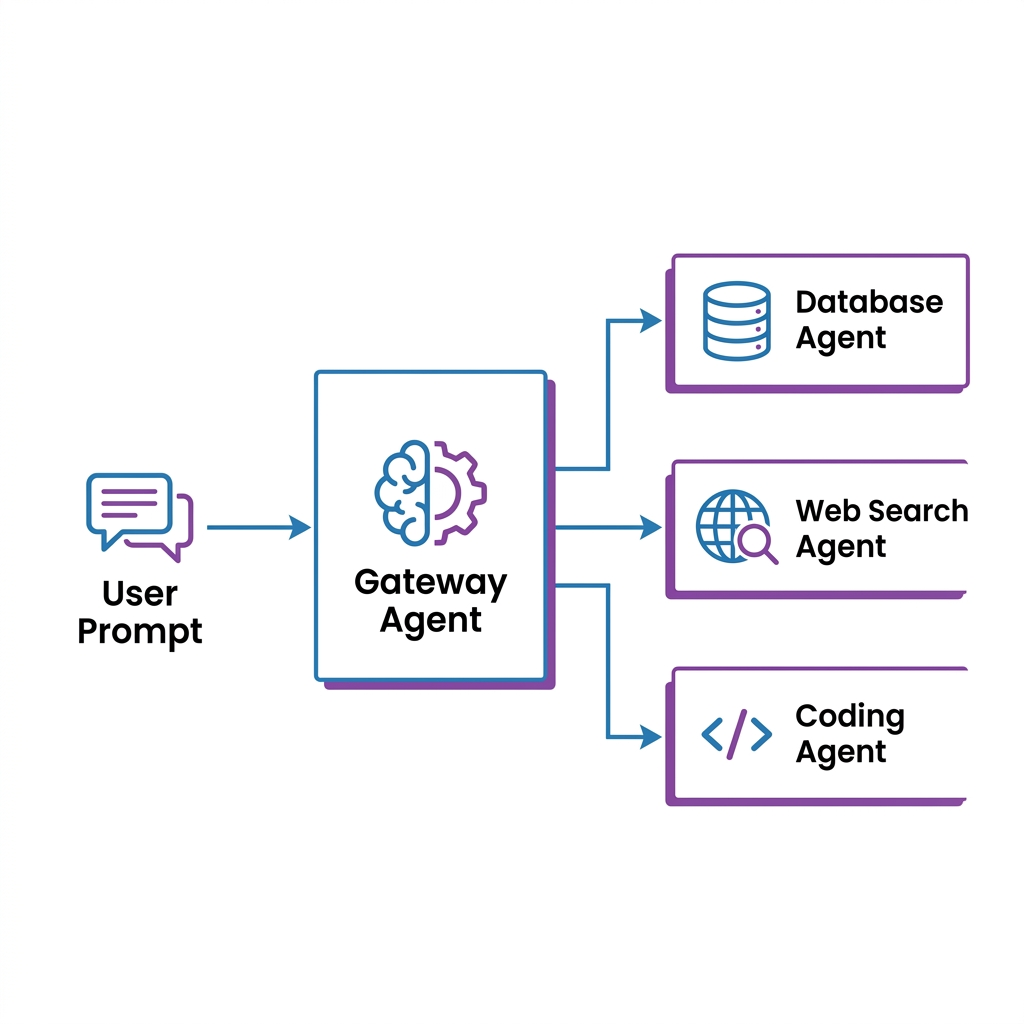
\includegraphics[width=0.85\textwidth]{../images/gateway_pattern.png}
    \caption{The Gateway Router Pattern for specialized sub-agents.}
    \label{fig:gateway_pattern}
\end{figure}

\section{Creating Tools \& Type Safety}
When we give an agent tools, we are giving it "hands and legs" to interact with the real world. However, LLMs hallucinate. If your tool expects a \texttt{Number} (like a User ID) but the LLM passes a \texttt{String} (like "John Doe"), your backend will crash.

\begin{concept}{Zod (The Bouncer)}
	Agent SDKs solve this by using data validation libraries like \textbf{Zod}. Zod acts as a bouncer at a club. Before the LLM is allowed to execute a tool, Zod checks its ID (the data types). If the LLM tries to pass a string instead of a number, Zod rejects it and tells the LLM to fix its mistake.
\end{concept}

\begin{codeblock}{Defining a Type-Safe Tool}{typescript}
import { z } from "zod";

const getWeatherTool = {
    name: "get_weather",
    description: "Fetches the current weather for a specific city.",
    parameters: z.object({
        city: z.string().describe("The name of the city, e.g., 'London'"),
        days: z.number().max(7).describe("Number of days for forecast")
    }),
    execute: async ({ city, days }) => {
        // Zod guarantees 'city' is a string and 'days' is a number <= 7
        return await fetchWeatherApi(city, days);
    }
};
\end{codeblock}

\section{Handoffs \& The "Lost Context" Bug}
When the Gateway Agent routes a task to a specialized agent, it is called a \textbf{Handoff}.

However, because these SDKs are still very new, there is a known bottleneck: \textbf{The Lost Context Bug}.
\begin{itemize}
	\item \textbf{The Bug:} When the Gateway Agent hands off a task to the Coding Agent, the Coding Agent finishes the task and returns the answer directly to the user. \textit{It forgets to hand control back to the Gateway Agent!} This breaks complex queries that require multiple agents.
	\item \textbf{The Quick Fix:} Instead of using the native Handoff function, treat your sub-agents as Tools using \texttt{agent.asTool()}. This forces the sub-agent to return its answer back to the Gateway Agent just like a normal tool call.
\end{itemize}

\begin{codeblock}{The "Agent as a Tool" Handoff Fix}{typescript}
// 1. Convert the specialized agent into a standard tool
const cookingAgentTool = cookingAgent.asTool();

// 2. Give that tool to the Gateway Agent
const gatewayAgent = new Agent({
    name: "Gateway Agent",
    instructions: "You are the router. Pass cooking questions to the cooking tool.",
    tools: [cookingAgentTool] // The Gateway can now invoke the sub-agent
});
\end{codeblock}

\section{Capstone: Autonomous Web Agents}
What if you want an agent to test a website or book a flight for you? We use tools like \textbf{Playwright} or \textbf{Selenium} to give the agent control of a real Chrome browser. Startups like \href{https://github.com/browser-use/browser-use}{Browser Use} have raised millions of dollars building open-source frameworks for this exact architecture!

The agent operates in a continuous \textbf{Perceive-Reason-Act} loop:
\begin{enumerate}
	\item \textbf{Plan (Reason):} The LLM analyzes the current state of the page and decides what to do next (e.g., "I need to click the Login button").
	\item \textbf{Execute (Act):} The Python/Node backend runs the Playwright script to click the specific DOM element or type text.
	\item \textbf{Observe (Perceive):} The system captures a screenshot of the browser to verify the page changed successfully, feeding it back to the LLM for the next loop.
\end{enumerate}

\begin{bestpractice}[Performance: Base64 Screenshots]
	Taking raw PNG screenshots and saving them to your hard drive during every loop is incredibly slow and will bottleneck your agent. Instead, capture the screenshot as a \textbf{Base64 Encoded String} in memory and pass that string directly to the LLM.
\end{bestpractice}

\chapter[Threads \& Guardrails]{Threads, Guardrails, \& Tracing\\in Agent SDK}

To move an agent from a local toy project to an enterprise production system, we must solve three major issues: Memory, Security, and Reliability.

\section{The Amnesia Problem (Threading)}
By default, LLM API calls are completely stateless. Once an agent finishes executing a task, it immediately forgets everything. If you tell an agent your name is "Harsh" and then ask "What is my name?" in the very next query, it will not know!

\begin{concept}{Checkpointing \& Threads}
	To fix this amnesia, we use \textbf{Threading}. Think of threading like saving a video game. We take the entire conversation history (what the user said, what tools were called, what the LLM replied) and save it to a database (like Postgres or Redis). Before executing the next user query, we "load the save file" and inject that history back into the agent so it remembers the context!
\end{concept}

\section{Security: The Bouncer Analogy}
Giving an AI access to production tools is incredibly dangerous. We must protect the system using \textbf{Guardrails}. Guardrails act like bouncers at a club, and they exist in two places:

\begin{itemize}
	\item \textbf{Input Guardrails (The Front Door Bouncer):} This bouncer checks the user's prompt \textit{before} the LLM even sees it.
	      \begin{itemize}
		      \item \textit{Example (Detect PII):} If an employee types their Social Security Number or personal email, the bouncer "trips the circuit" and throws an exception to protect their privacy.
		      \item \textit{Example (Prompt Injection):} If a user types malicious spoofing commands (e.g., "Disregard previous instructions"), the bouncer rejects the input.
	      \end{itemize}
	\item \textbf{Output Guardrails (The Back Door Bouncer):} This bouncer checks the LLM's generated response \textit{before} showing it to the user.
	      \begin{itemize}
		      \item \textit{Example (Competitor Check):} If you build a customer service bot for Samsung, and the LLM hallucinates an insult about Apple, Apple could sue! The back door bouncer blocks the message to prevent legal disasters.
	      \end{itemize}
\end{itemize}

\begin{tipbox}[Parallel Execution]
	Guardrails are usually small, fast SLMs (Small Language Models). To prevent your app from becoming slow, always execute multiple guardrails simultaneously using \texttt{run\_parallel=true}.
\end{tipbox}

\section{Human-in-the-Loop (HITL)}
Even with excellent guardrails, LLMs make mistakes. For highly destructive operations (e.g., executing a \texttt{DROP TABLE} SQL command, or formatting a hard drive), we introduce the ``Red Button''---\textbf{Human-in-the-Loop (HITL)}.

When an agent wants to use a destructive tool, it pauses its execution loop and explicitly asks a human for permission ("Are you sure you want me to execute this?"). The tool only runs if the human clicks Yes.

\section{Tracing \& Observability}
In production, every agent execution must be logged. Agent SDKs provide built-in \textbf{Tracing} dashboards. These dashboards allow developers to monitor exactly how much time an operation took (latency), how much money it cost (token count), and exactly which tools were triggered behind the scenes.
\chapter{Memory Systems in AI Agents}

If an LLM is a powerful brain, the \textbf{Context Window} is its extremely limited short-term memory. We cannot achieve AGI (Artificial General Intelligence) if our AI constantly forgets its past.

\section{The Context Limit (Sliding Window)}
Why don't we just append the entire chat history forever? Because context windows are finite. If we push too many tokens, we experience severe latency spikes and extreme hallucinations.

Instead, developers use a \textbf{Sliding Window}. Imagine a conveyor belt: as new messages are added to the front, the oldest messages fall off the back and are forgotten forever. To solve this amnesia, modern production systems require a dedicated \textbf{Memory Layer}.

\begin{figure}[!ht]
    \centering
    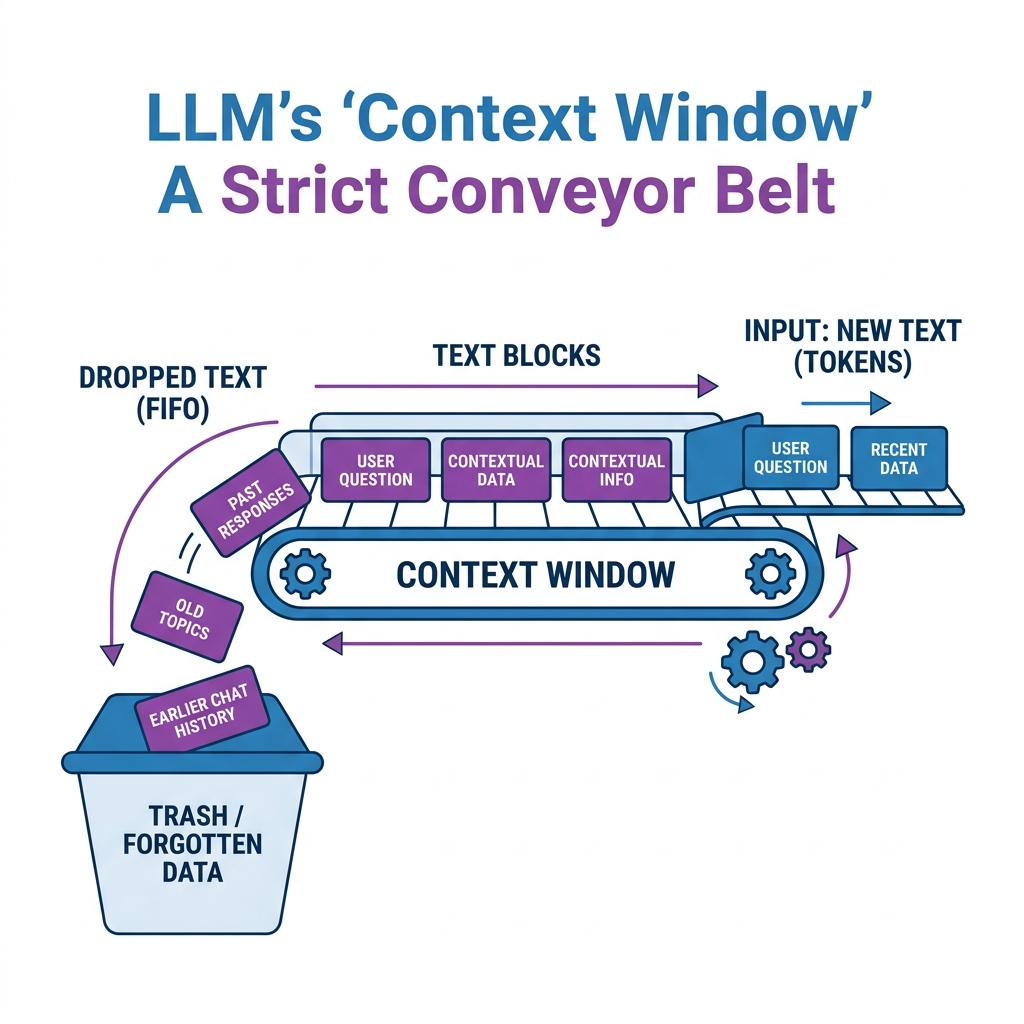
\includegraphics[width=\textwidth]{../images/conveyor_belt.png}
    \caption{The Context Window visualized as a strictly sized Conveyor Belt (FIFO Memory).}
    \label{fig:conveyor_belt}
\end{figure}

\section{Short-Term vs. Long-Term Memory}
To solve the sliding window problem, we mimic human cognition by splitting memory into two categories:

\begin{itemize}
	\item \textbf{Short-Term Memory:} The immediate conversation (e.g., the last 50 messages). This is stored in an ultra-fast cache like \textbf{Redis}. This is a solved problem.
	\item \textbf{Long-Term Memory:} Knowledge that persists across days, months, or years. This is the hard problem, and it is categorized into three buckets:
	      \begin{itemize}
		      \item \textbf{Factual Memory:} Hard facts scoped to a specific user (e.g., "User's name is Harsh").
		      \item \textbf{Episodic Memory:} Inferred behavioral patterns based on past events (e.g., "User consistently ignores examples related to politics").
		      \item \textbf{Semantic Memory:} Generalized facts applicable to everyone (e.g., "Scaler pricing plans").
	      \end{itemize}
\end{itemize}

\begin{concept}{The Implementation (Mem0 AI)}
	How does a production tool like Mem0 actually build this?
	\begin{enumerate}
		\item \textbf{The Queue \& The Judge:} Every message is pushed to a background Queue. An \textbf{LLM Judge} reads each message using Few-Shot Prompting and decides: \textit{"Is there a long-term fact hidden in this text?"}
		\item \textbf{Vector Storage:} If a fact is found (e.g., "My name is John"), it is converted into an embedding and stored in a Vector Database (like Qdrant or Postgres pgvector), tightly tagged with the \texttt{user\_id}.
		\item \textbf{Context Injection:} When the user logs in the next day, the system does a Vector Similarity Search, pulls all relevant facts from the database, and injects them directly into the \textbf{System Prompt}. The agent is now "Memory-Aware"!
	\end{enumerate}
\end{concept}

\chapter{Graph Databases \& Relational Memory}

While Vector Databases (like Qdrant) are excellent at finding semantic similarity, they have a massive blind spot: they cannot understand \textbf{Relationships}.

\section{The Bottleneck of Vector DBs}
Vector Databases fail at \textbf{Relationship Traversal}.

\begin{concept}{The Legal Document Analogy}
	Imagine a massive legal contract. On Page 1, it says: \textit{"Please refer to Clause 46."} The actual details of Clause 46 are located on Page 256.

	If a user asks an AI, "Tell me about Clause 46", a Vector Database will do a string match and return Page 1. It fails completely to traverse the reference and fetch the actual information on Page 256. It lacks relational context.
\end{concept}

\section{Graph Database Fundamentals}
To solve this, we use \textbf{Graph Databases} (e.g., Neo4j). In a graph database, data isn't stored in tables or vectors; it is stored as a web of connections.

\begin{itemize}
	\item \textbf{Nodes (The Nouns):} Entities like People, Places, or Organizations. (e.g., Node: MSD, Node: Virat).
	\item \textbf{Edges (The Verbs):} Directed lines connecting the nodes that define the relationship. (e.g., MSD \texttt{[:FOLLOWS]} Virat).
\end{itemize}

\begin{tipbox}[Social Media Analogy]
	All major social media recommendation algorithms run on Graph Databases. This is how the "Celebrity Problem" is solved. When MSD hits the follow button on Virat Kohli's profile, a directed edge is created between their two nodes.
\end{tipbox}

\section{The Enterprise IT Analogy}
Why does an AI Agent need a Graph DB? Consider a corporate HR chatbot.

If a user says, \textit{"My laptop is broken,"} the agent needs to find someone to help. With a Graph DB, the agent can traverse the network to find the \texttt{[IT\_Support]} node, traverse the \texttt{[:WORKS\_AT]} edges connected to that node, find three specific employees, and route the ticket to one of them. The AI is leveraging relationships to solve problems.

\section{The Tradeoff: Why it's Deprecated}
Despite being incredibly powerful for contextual relationships, Graph Databases have a major production flaw: \textbf{Traversing a massive graph is computationally expensive and very slow.}

Because of this severe latency cost, modern Memory Layers (like recent versions of Mem0) have actually \textbf{deprecated} graph databases. They have reverted to highly optimized Vector Searches instead. You should only implement a Graph Database if relational mapping is the primary product feature (like building a social network).

\begin{codeblock}{Cypher Query Example}{sql}
	-- Cypher is the query language for Neo4j (Often written by the LLM itself)
	-- Match a Person entity working at the "Scaler" Organization
	MATCH (p:Person)-[:WORKS_AT]->(o:Organization {name: "Scaler"})
	RETURN p.name
\end{codeblock}

\begin{tipbox}
	You rarely need to write complex Cypher queries manually. Because graph databases have a rigid schema, LLMs are highly proficient at translating natural language into valid Cypher queries dynamically.
\end{tipbox}

\section{Hybrid Knowledge Graphs}
In complex Agentic systems (like HR or Legal Tech), developers implement a \textbf{Hybrid RAG} approach. The Agent queries the Vector DB to retrieve textual semantic matches and simultaneously queries the Graph DB to traverse hierarchical or referenced relationships.

\chapter[Conversational \& Voice AI]{Conversational \& Voice-Based\\AI Agents}

Building Voice-to-Voice AI agents is significantly more complex than text-based agents due to the nature of audio waves, latency requirements, and stateful streaming protocols.

\section{The Legacy Voice Pipeline}
Before native voice-to-voice models existed, developers used a chained, modular approach.
\begin{enumerate}
	\item \textbf{Speech-to-Text (STT):} The user's audio was captured (e.g., via browser APIs or AssemblyAI) and transcribed.
	\item \textbf{Text-to-Text (LLM):} The transcribed text was passed to a standard LLM to generate a text response.
	\item \textbf{Text-to-Speech (TTS):} The LLM's text output was converted back into an audio file (e.g., using OpenAI's TTS) and streamed back to the user.
\end{enumerate}

\begin{warningbox}[The Bottleneck of Legacy Pipelines]
	This approach introduces severe \textbf{latency}. Transcribing, generating text, and synthesizing audio consecutively makes conversational flow unnatural. Furthermore, routing audio files through a backend Node.js server causes the server to choke under heavy load.
\end{warningbox}

\section[Native WebRTC \& LiveKit]{Modern Architecture:\\Native WebRTC \& LiveKit}
Modern voice models (e.g., GPT-4o Realtime API) are native \textbf{Speech-to-Speech} transformers. They bypass the STT/TTS conversion, significantly reducing latency.
These models stream audio via \textbf{WebRTC}. However, scaling WebRTC connections is notoriously difficult. Consequently, providers like OpenAI integrate with third-party infrastructure platforms (e.g., \textbf{LiveKit}) to handle WebRTC connection scaling under the hood.

\section{The Remote Proxy Pattern (Ephemeral Tokens)}

To prevent backend servers from choking on audio buffers, clients (e.g., a Next.js frontend) must establish a direct WebRTC connection with the OpenAI/LiveKit servers. However, we cannot expose our secret OpenAI API key on the frontend.

\begin{concept}{Ephemeral Token Exchange}
	To solve this, we use the \textbf{Remote Proxy Pattern}:
	\begin{enumerate}
		\item \textbf{Request:} The Next.js frontend sends a request to the backend server.
		\item \textbf{Negotiation:} The backend securely uses the secret API key to request an \textit{Ephemeral Token} (a short-lived, permission-scoped token) from the OpenAI server.
		\item \textbf{Delivery:} The backend returns this Ephemeral Token to the frontend.
		\item \textbf{Direct Connection:} The frontend uses the Ephemeral Token to establish a direct WebRTC session with the OpenAI voice model, bypassing the backend entirely for audio transmission.
	\end{enumerate}
\end{concept}

\begin{tipbox}[The Corporate Visitor Analogy]
	Think of the OpenAI API Key as a \textbf{Master Key} to a high-security corporate vault. You would never give the Master Key to a random visitor (the frontend client). Instead, the visitor goes to the front desk (the backend), and the receptionist uses the Master Key to print a \textbf{Temporary Visitor Badge} (Ephemeral Token). The visitor can then use this badge to access specific rooms for the next 30 minutes, without ever seeing or holding the Master Key.
\end{tipbox}

\begin{figure}[!ht]
    \centering
    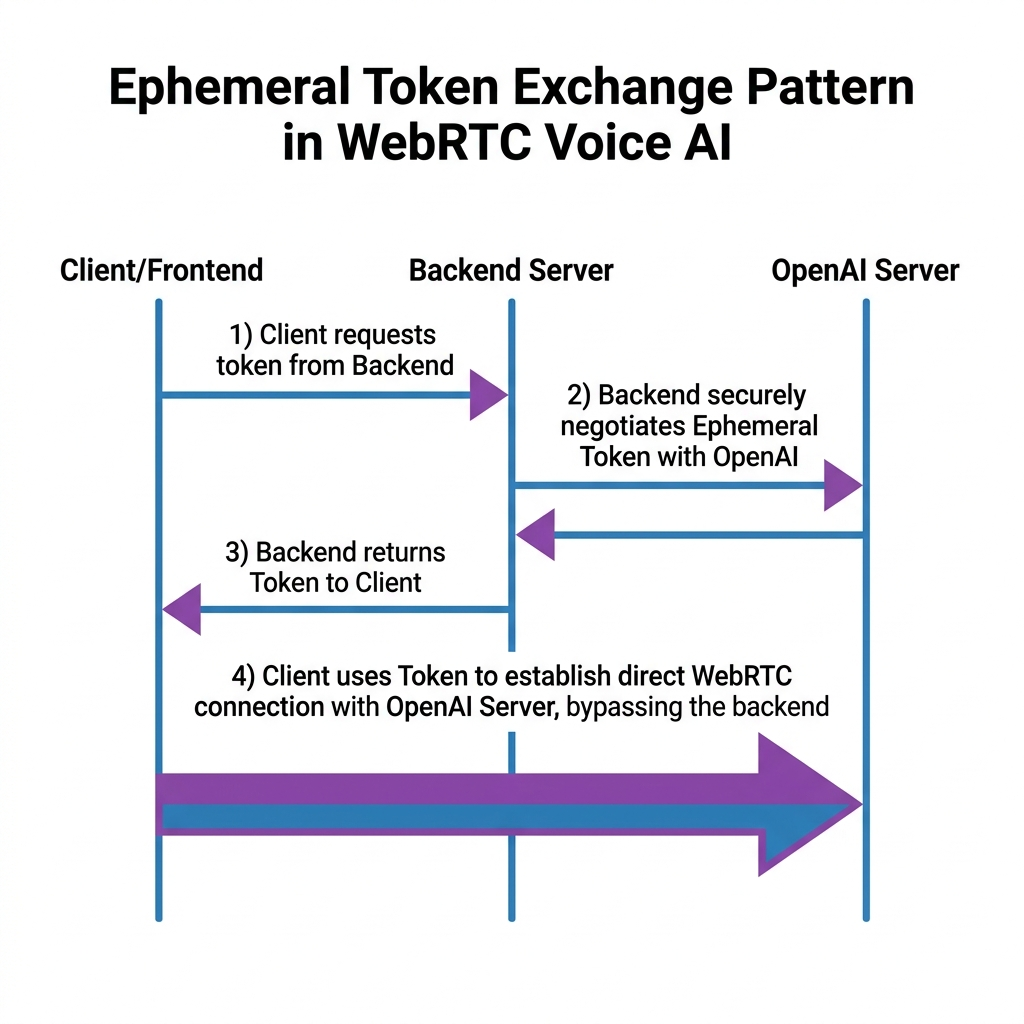
\includegraphics[width=\textwidth]{../images/ephemeral_token.png}
    \caption{Ephemeral Token Exchange sequence bypassing backend bottlenecks.}
    \label{fig:ephemeral_token}
\end{figure}

\chapter{Model Context Protocol (MCP)}

Historically, every AI provider (OpenAI, Anthropic, Google) had a proprietary JSON format for defining tools. A tool written for OpenAI's SDK could not be easily ported to Gemini or Claude.

Anthropic introduced the \textbf{Model Context Protocol (MCP)} to solve this. MCP acts like the HTTP of AI tools---it provides a universal, standardized schema. If a tool is built as an MCP server, any MCP-compatible LLM can interface with it.

\begin{tipbox}[The Universal USB-C Analogy]
	Before MCP, integrating tools with LLMs was like the early days of smartphones: OpenAI required an "Apple Lightning" cable, Anthropic required a "Micro-USB" cable, and Gemini required a proprietary charger. MCP is the equivalent of introducing the \textbf{USB-C standard}. Now, as long as a data source or tool is built as an MCP Server (has a USB-C port), any LLM (Client) can plug into it effortlessly.
\end{tipbox}

\section{MCP Architecture}
The protocol decouples the AI model from the tool execution environment using three layers:
\begin{itemize}
	\item \textbf{MCP Client:} The interface the user interacts with (e.g., Cursor IDE, Claude Desktop).
	\item \textbf{MCP Server:} The backend process containing the actual tool logic (e.g., a server that queries a PostgreSQL database or buys/sells stocks).
	\item \textbf{MCP Host:} A middleware layer. The Client never talks directly to the Server; it communicates via the Host to negotiate capabilities.
\end{itemize}

\begin{figure}[!ht]
    \centering
    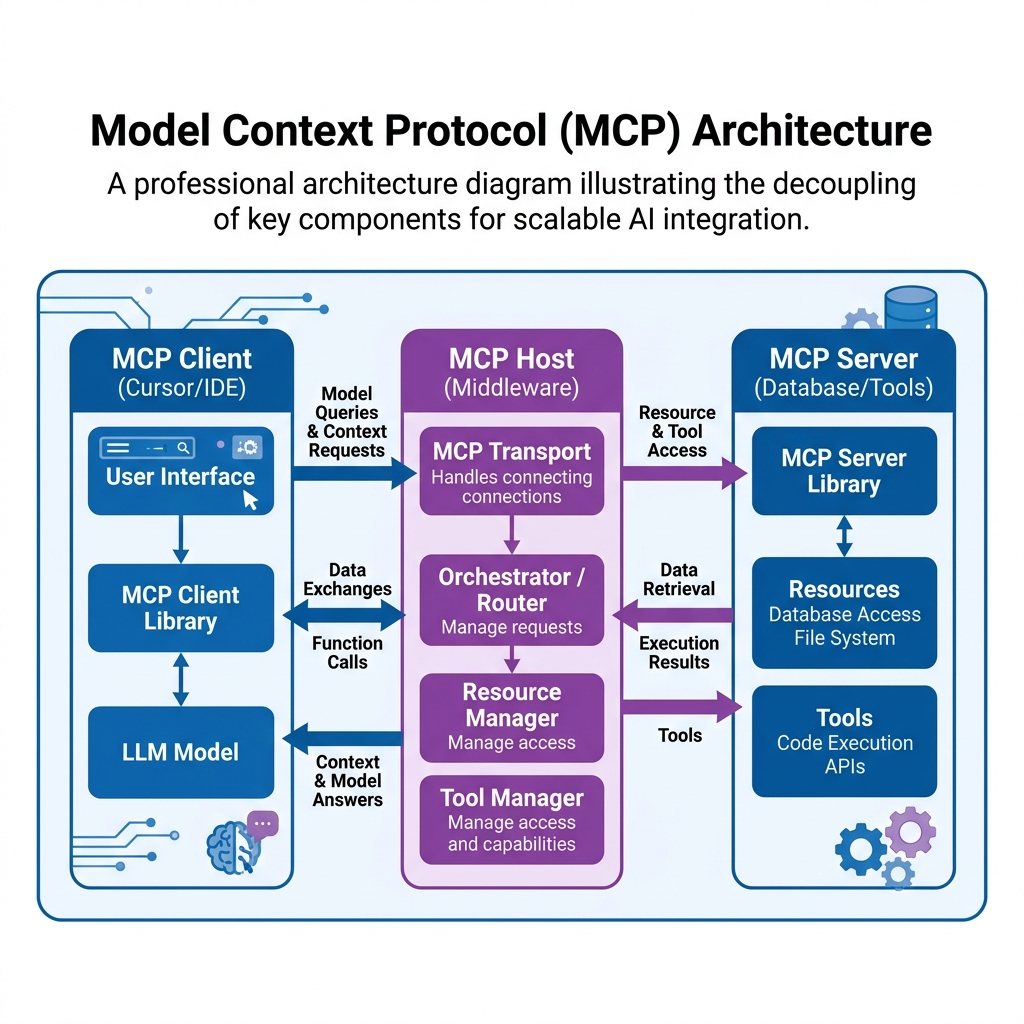
\includegraphics[width=\textwidth]{../images/mcp_architecture.png}
    \caption{Model Context Protocol decoupled architecture.}
    \label{fig:mcp_architecture}
\end{figure}

\section{Transport Layers}
MCP servers require a transport layer to receive requests.
\begin{itemize}
	\item \textbf{Local Communication (\texttt{stdio}):} For local servers, MCP uses Standard IO. The terminal is blocked, acting as a pipe.
	\item \textbf{Remote Communication:} Handled via HTTP and Server-Sent Events (SSE).
\end{itemize}

\begin{warningbox}[Architectural Shift: Stateful vs Stateless]
	Version 1 of MCP was \textbf{stateful}, requiring persistent connections (SSE) which made scaling difficult and costly. Version 2 of MCP (releasing July 2026) marks a paradigm shift to a \textbf{stateless} HTTP architecture to improve reliability and reduce infrastructure overhead.
\end{warningbox}

\chapter{Deployment, Scaling \& Infrastructure}
Deploying a Generative AI application involves traditional backend scaling combined with AI-specific considerations, particularly around third-party rate limiting.

\section{The Rate Limiting Bottleneck}
Assume your server can handle 1 million concurrent users. If those users simultaneously trigger an LLM feature, your server will forward 1 million requests to OpenAI. OpenAI will immediately enforce its \textbf{Rate Limits} (e.g., max 100 requests/sec or max tokens/sec), causing your entire system to crash.

\begin{tipbox}
	\textbf{Solution: Queuing Services.} Never make direct LLM API calls synchronously from the client request. Implement a Push/Pull Queue (e.g., AWS SQS, RabbitMQ, Kafka). Enqueue the user requests and let background workers dequeue and process them at a rate that stays safely below the LLM provider's rate limits.
\end{tipbox}

\begin{tipbox}[The Nightclub Bouncer Analogy]
	Think of the OpenAI API as an exclusive nightclub with a strict bouncer. If 1,000 people try to rush the door simultaneously (synchronous direct calls), the bouncer will completely shut down the club (Rate Limit Error / Server Crash). A Queuing Service acts like the \textbf{velvet rope queue} outside, ensuring people are let in steadily at a manageable pace (e.g., 50 per second), keeping the club running smoothly.
\end{tipbox}

\begin{infobox}[The Harness Layer]
	In production, rate limiting and API orchestration are often abstracted away using a \textbf{Harness Layer}. This is an extra infrastructure wrapper surrounding the autonomous agent, providing a unified interface for database connections, queue management, and external API safeguards.
\end{infobox}

\section{Zero-Downtime Deployment Strategies}
Updating an AI application by stopping the server, updating the code, and restarting causes unacceptable downtime. DevOps teams use zero-downtime strategies:

\begin{enumerate}
	\item \textbf{Blue-Green Deployment:} You have a live server (V0). You spin up an entirely new server (V1). Once V1 is fully tested and healthy, you instantly redirect all traffic from V0 to V1. Finally, you destroy V0.
	\item \textbf{Rolling Updates:} If you have a cluster of servers, you incrementally upgrade a few servers to V1 at a time, gradually shifting traffic over until all servers are updated.
\end{enumerate}

\begin{tipbox}[The Highway Analogy]
	Blue-Green deployment is like needing to change a car on the highway without stopping. Instead of pulling over (downtime), you drive a brand new car (Green) directly next to the old one (Blue), jump across while moving at 60mph, and then let the old car veer off the road. The passengers (users) never experienced a stop.
\end{tipbox}

\section{AWS Infrastructure Security}
When spinning up remote machines (e.g., AWS EC2), they are entirely isolated by default.
\begin{itemize}
	\item \textbf{Security Groups:} Act as virtual firewalls.
	\item \textbf{Inbound Rules:} Control who can access your machine (e.g., allowing SSH on Port 22 strictly from your company's IP address, or HTTP on Port 80).
	\item \textbf{Outbound Rules:} Control where your machine can send requests (e.g., allowing requests to \texttt{api.openai.com}).
\end{itemize}

Beyond Security Groups, VPS providers often configure a \textbf{NACL (Network Access Control List)}. While Security Groups operate at the instance level, NACL operates at the subnet level, providing an additional stateless layer of database and network isolation. For comprehensive security documentation, refer to the \href{https://docs.aws.amazon.com/vpc/latest/userguide/VPC_Security.html}{AWS VPC Security Guide}.

\begin{warningbox}[Production Standard: Load Balancers]
	Never expose your EC2 instance directly to the public internet. Keep the EC2 machine inside a Private Subnet. Expose a \textbf{Load Balancer} (or an Nginx reverse proxy) to the public, which forwards requests securely to your isolated application server.
\end{warningbox}

\begin{figure}[!ht]
    \centering
    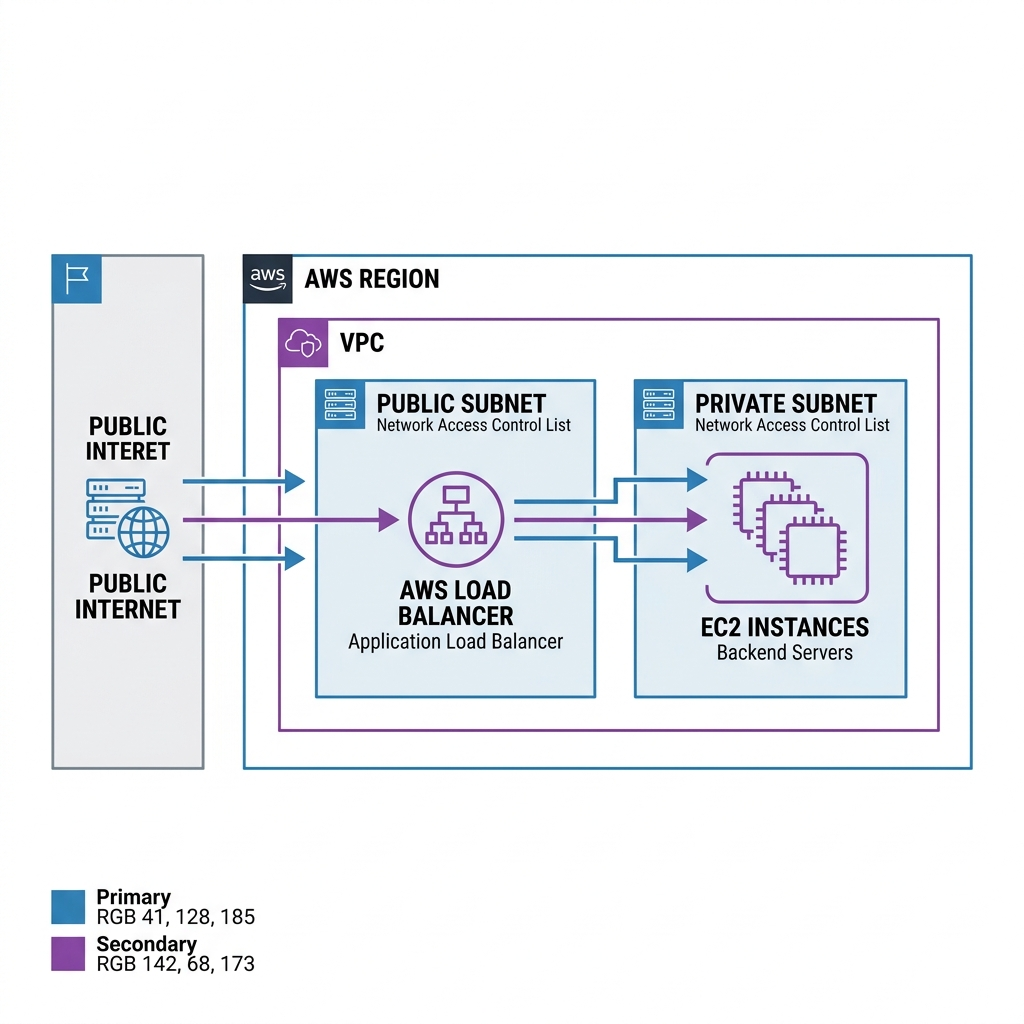
\includegraphics[width=\textwidth]{../images/vpc_loadbalancer.png}
    \caption{Production standard AWS VPC Architecture with public Load Balancers and private backend instances.}
    \label{fig:vpc_loadbalancer}
\end{figure}

\section{EC2 \& Dockerized Nginx Logistics}
When interacting with raw AWS EC2 instances, secure access and containerized reverse proxies are standard.

\begin{codeblock}{EC2 SSH Access \& Docker Setup}{bash}
	# 1. Secure your private key (required for AWS SSH)
	chmod 400 genai.pem

	# 2. Connect to the EC2 instance (Default port 22)
	ssh -i genai.pem ubuntu@<PUBLIC_IP>

	# 3. Install Docker
	sudo apt update
	sudo apt install docker.io

	# 4. Run Nginx as a proxy container
	sudo docker run -p 80:80 nginx
\end{codeblock}
For more container deployment patterns, see the \href{https://docs.docker.com/}{Docker Documentation}.

\begin{warningbox}[EC2 Billing Warning - Terminate and Do Not Stop]
	When working on your final projects, \textbf{always terminate} your AWS EC2 instances when you are finished. Simply "stopping" an instance still incurs costs for the EBS volume (storage) attached to it. Terminate instances to fully destroy the resources and prevent unexpected AWS billing charges.
\end{warningbox}

\chapter{Academic \& Project Reminders}

To successfully complete the GenAI engineering module, please note the following critical deadlines for your assignments:

\section{Deadlines \& Vivas}
\begin{itemize}
	\item \textbf{Group Project Deadline:} Extended to \textbf{June 18, 2026}. Ensure all your code is merged, deployed, and functional by this date.
	\item \textbf{Project Vivas:} Scheduled between \textbf{June 21 and June 30, 2026}. Be prepared to defend your architectural decisions (e.g., why you chose a vector DB over a graph DB, or how you implemented MCP).
\end{itemize}

\end{document}
